\documentclass[6pt]{article}
\usepackage[utf8]{inputenc}
\usepackage[margin=1in]{geometry}
\usepackage{lastpage}
\usepackage{fancyhdr}
\usepackage{tikz}
\usepackage{pgfplots}
\usetikzlibrary{arrows}
\usepackage{multicol}
\usepackage{tabularx}
\usepackage{adjustbox}
\usepackage{color}
\usepackage{listings}
\usepackage{graphicx}
\usepackage{verbatim}
\usepackage{mathtools} 
\usepackage{amssymb}
\usepackage{amsmath}
\usepackage{algorithm}
\usepackage{algpseudocode}
\usepackage{url}
\usepackage{hyperref}
\usepackage{caption}

\pagestyle{fancy}
\lhead{Blaney}
\chead{\textit{Algorithm Analysis - Spring 2014}}
\rhead{Homework 3}
\cfoot{\thepage\ of \pageref{LastPage}}

\setlength{\parindent}{0pt}

\definecolor{deepblue}{rgb}{0,0,0.5}
\definecolor{deepred}{rgb}{0.6,0,0}
\definecolor{deepgreen}{rgb}{0,0.5,0}
\definecolor{deeppurple}{rgb}{0.6,0,0.5}
\definecolor{deepgray}{rgb}{0.5,0.5,0.5}

\lstset{ %
  backgroundcolor=\color{white},   % choose the background color; you must add \usepackage{color} or \usepackage{xcolor}
  basicstyle=\ttfamily\footnotesize,        % the size of the fonts that are used for the code
  breakatwhitespace=false,         % sets if automatic breaks should only happen at whitespace
  breaklines=true,                 % sets automatic line breaking
  captionpos=b,                    % sets the caption-position to bottom
  commentstyle=\color{deepgreen},    % comment style
  deletekeywords={},            % if you want to delete keywords from the given language
  escapeinside={\%*}{*)},          % if you want to add LaTeX within your code
  extendedchars=true,              % lets you use non-ASCII characters; for 8-bits encodings only, does not work with UTF-8
  frame=none,                    % adds a frame around the code
  keepspaces=true,                 % keeps spaces in text, useful for keeping indentation of code (possibly needs columns=flexible)
  keywordstyle=\color{deepblue},       % keyword style
  language=Python,                   % the language of the code
  otherkeywords={self,True,False,None},            % if you want to add more keywords to the set
  emph={IDS,DFS,improved_DFS,improved_IDS,__init__},          % Custom highlighting
  emphstyle=\color{deepred},    % Custom highlighting style
  numbers=left,                    % where to put the line-numbers; possible values are (none, left, right)
  numbersep=5pt,                   % how far the line-numbers are from the code
  numberstyle=\ttfamily\tiny\color{deepgray}, % the style that is used for the line-numbers
  rulecolor=\color{black},         % if not set, the frame-color may be changed on line-breaks within not-black text (e.g. comments (green here))
  showspaces=false,                % show spaces everywhere adding particular underscores; it overrides 'showstringspaces'
  showstringspaces=false,          % underline spaces within strings only
  showtabs=false,                  % show tabs within strings adding particular underscores
  stepnumber=1,                    % the step between two line-numbers. If it's 1, each line will be numbered
  stringstyle=\color{deepred},     % string literal style
  tabsize=2,                       % sets default tabsize to 2 spaces
}

\title{CS319}
\author{Jim Blaney}
\date{February 27, 2014}

\begin{document}
\setlength{\abovecaptionskip}{0pt}
\setlength{\belowcaptionskip}{5pt}

\noindent I pledge that I have neither given nor received any unauthorized aid on this assignment. \\[4em]
%\-\hspace{0.55\linewidth} \includegraphics[height=4em]{signature-latex}

\section*{Input Data}
\begin{minipage}{0.5\textwidth}
\subsection*{Graph}
\end{minipage}
\begin{minipage}{0.5\textwidth}
\subsection*{Adjacency Matrix}
\end{minipage}

\adjustbox{valign=t}{
\begin{minipage}{0.5\textwidth}
\begin{figure}[H]
%\begin{center}
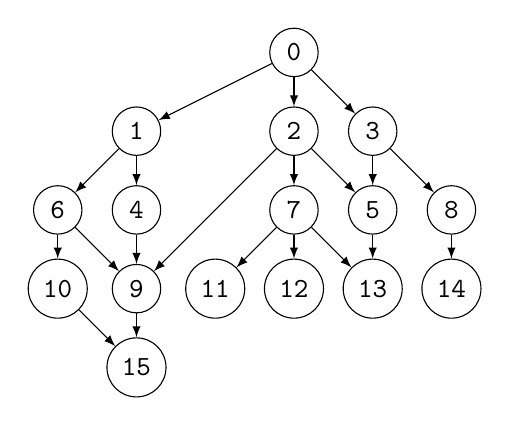
\begin{tikzpicture}[->,>=latex,auto,node distance=2.5cm,main node/.style={circle,draw,font=\ttfamily}]

  \foreach \place/\x in {
    {(3,4)/0},
    {(1,3)/1}, 
    {(3,3)/2},
    {(4,3)/3},
    {(1,2)/4}, 
    {(4,2)/5}, 
    {(0,2)/6}, 
    {(3,2)/7}, 
    {(5,2)/8},
    {(1,1)/9},
    {(0,1)/10},
    {(2,1)/11},
    {(3,1)/12},
    {(4,1)/13},
    {(5,1)/14},
    {(1,0)/15}}
  \node[main node] (\x) at \place {\x};
  
  \path[every node/.style={font=\small}]
    (0) edge (1)
    (0) edge (2)
    (0) edge (3)
    (1) edge (4)
    (1) edge (6)
    (2) edge (5)
    (2) edge (7)
    (2) edge (9)
    (3) edge (5)
    (3) edge (8)
    (4) edge (9)
    (5) edge (13)
    (6) edge (9)
    (6) edge (10)
    (7) edge (11)
    (7) edge (12)
    (7) edge (13)
    (8) edge (14)
    (9) edge (15)
    (10) edge (15);
\end{tikzpicture}
%\end{center}
\end{figure}
\end{minipage}
}
\adjustbox{valign=t}{
\begin{minipage}{0.5\textwidth}
\begin{figure}[H]
%\begin{center}
\texttt{0,1,1,1,0,0,0,0,0,0,0,0,0,0,0,0 \\
0,0,0,0,1,0,1,0,0,0,0,0,0,0,0,0 \\
0,0,0,0,0,1,0,1,0,1,0,0,0,0,0,0 \\
0,0,0,0,0,1,0,0,1,0,0,0,0,0,0,0 \\
0,0,0,0,0,0,0,0,0,1,0,0,0,0,0,0 \\
0,0,0,0,0,0,0,0,0,0,0,0,0,1,0,0 \\
0,0,0,0,0,0,0,0,0,1,1,0,0,0,0,0 \\
0,0,0,0,0,0,0,0,0,0,0,1,1,1,0,0 \\
0,0,0,0,0,0,0,0,0,0,0,0,0,0,1,0 \\
0,0,0,0,0,0,0,0,0,0,0,0,0,0,0,1 \\
0,0,0,0,0,0,0,0,0,0,0,0,0,0,0,1 \\
0,0,0,0,0,0,0,0,0,0,0,0,0,0,0,0 \\
0,0,0,0,0,0,0,0,0,0,0,0,0,0,0,0 \\
0,0,0,0,0,0,0,0,0,0,0,0,0,0,0,0 \\
0,0,0,0,0,0,0,0,0,0,0,0,0,0,0,0 \\
0,0,0,0,0,0,0,0,0,0,0,0,0,0,0,0 \\
}
%\end{center}
\end{figure}

\end{minipage}
}\\[1em]

\section*{Data Structures}

\subsection*{Graph}

Python:
\begin{lstlisting}[language=Python]
class Graph:
    def __init__(self, num_vertices = 0):
        self.p = [[0 for x in range(num_vertices)] for x in range(num_vertices)];

    def get_adjacent(self, i):
        return [x for x in xrange(self.num_nodes()) if self.p[i][x] != 0];

    def is_edge(self, i, j):
        return self.p[i][j] != 0;

    def num_nodes(self):
        return len(self.p[0]);
        
    def set_edge(self, i, j, value):
        self.p[i][j] = value;
\end{lstlisting}

\subsection*{Discussion}

For all of the homework problems, I implemented and made use of the simple graph specification (CS 319 Lecture 7, Slide 5). I also added a convenience method, \lstinline{get_adjacent}, which queries the internal edge matrix for a particular node to find adjacent node indices. For stack and queue structures, the Python \lstinline{list} contains the functions necessary to avoid deep implementation.

\pagebreak
\section*{Problem 1 [COMPLETE]}

\subsection*{Implementation}

Python:
\begin{lstlisting}[language=Python]
def DFS(graph, vertex = 0, visited = None, depth = -1):

    if visited is None:
        visited = [False for x in xrange(graph.num_nodes())];

    if not visited[vertex]:
        visited[vertex] = True;
        sys.stdout.write(str(vertex) + " ");

    for adjacent in graph.get_adjacent(vertex):
        if adjacent is vertex:
            continue;
        if depth != 0 and not visited[adjacent]:
            DFS(graph, adjacent, visited, depth - 1);
\end{lstlisting}


\subsection*{Output}

\begin{lstlisting}
0 1 4 9 15 6 10 2 5 13 7 11 12 3 8 14
\end{lstlisting}
 \ \\
\section*{Problem 2 [COMPLETE]}

\subsection*{Implementation}

Python:
\begin{lstlisting}[language=Python]
def DFS(graph, vertex = 0, visited = None, depth = -1):

    if visited is None:
        visited = [False for x in xrange(graph.num_nodes())];

    if not visited[vertex]:
        visited[vertex] = True;
        sys.stdout.write(str(vertex) + " ");

    for adjacent in graph.get_adjacent(vertex):
        if adjacent is vertex:
            continue;
        if depth != 0:
            DFS(graph, adjacent, visited, depth - 1);

def IDS(graph):

    visited = [False for x in xrange(graph.num_nodes())];

    for depth in xrange(graph.num_nodes()):
        if all(visited):
            break;
        DFS(graph, 0, visited, depth);
\end{lstlisting}


\subsection*{Output}

\begin{lstlisting}
0 1 2 3 4 6 5 7 9 8 10 13 11 12 15 14
\end{lstlisting}

\section*{Problem 3 [COMPLETE]}

\subsection*{Implementation}

Python:
\begin{lstlisting}[language=Python]
def improved_DFS(graph, vertex = 0, visited = None, depth = -1):

    if visited is None:
        visited = [False for x in range(graph.num_nodes())];

    if not visited[vertex]:
        visited[vertex] = True;
        sys.stdout.write(str(vertex) + " ");

    memory = [];

    for adjacent in graph.get_adjacent(vertex):
        if adjacent is vertex:
            continue;
        if depth != 0:
            memory.extend(improved_DFS(graph, adjacent, visited, depth - 1));
        elif not visited[adjacent]:
            memory.append(adjacent);

    return memory;

def improved_IDS(graph, vertex = 0):

    visited = [False for x in range(graph.num_nodes())];
    memory = [vertex];

    if not all(visited):
        while len(memory) > 0:
            memory.extend(improved_DFS(graph, remembered_vertices.pop(0), visited, 0));
            memory = unique(memory);
\end{lstlisting}

\subsection*{Output}

\begin{lstlisting}
0 1 2 3 4 6 5 7 9 8 10 13 11 12 15 14
\end{lstlisting}

\end{document}
